\chapter[Introdução]{Introdução}

O aumento da capacidade de armazenamento e processamento de dados tem possibilitado o desenvolvimento de sistemas inteligentes através do aprendizado de máquina. Tal desenvolvimento, por sua vez, permitiu avanços em diversas áreas da computação, microeletrônica e sensoriamento. 

Hoje, aplicações tais como pesquisas web, sistemas \textit{anti-spam}, reconhecimento de voz, recomendações de produto e diversas outras são frutos desse progresso. Porém a disponibilidade de quantidades massivas de dados, apresenta não só um horizonte vasto de possíveis aplicações, mas também desafios para seleção e processamento desses dados.


\section{Aprendizado de Máquina}

Aprendizado de máquina é o campo da computação responsável por desenvolver e empregar sistemas ou modelos que, através da sua exposição à experiências, são capazes de melhorar sua performance na realização de determinada tarefa \cite{mitchell_1997}.

O processo de desenvolvimento de modelos com aprendizado de máquina pode ser dividido, em linhas gerais, em duas grandes etapas. 

Inicialmente os dados disponíveis são analisados e tratados. Nessa etapa procura-se identificar correlações entre as informações disponíveis e as variáveis de interesse. Além disso, são explorados possíveis filtros, transformações e outros algoritmos que possam facilitar o aprendizado do modelo. Também é necessário realizar nessa etapa a separação dos dos dados que serão utilizados para treinamento, validação e teste no decorrer do processo.

Na etapa seguinte objetiva-se obter um modelo capaz de reproduzir o comportamento do sistema que gerou o conjunto de dados. Para tal, um ou mais modelos e algoritmos são selecionados e o treinamento é realizado. Duas características são de fundamental importância e devem ser controladas: a capacidade de assimilação do comportamento representado pelos dados (complexidade) e a capacidade de extrapolação das saídas para novas entradas (generalização).


\begin{figure}[H]
    \caption{\textcolor{red}{ADAPTAR:} Fluxo de desenvolvimento de sistemas inteligentes. }
    \begin{center}
    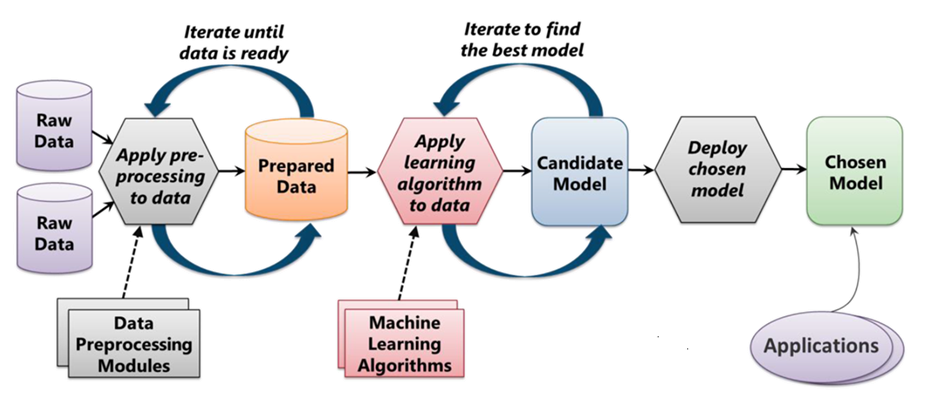
\includegraphics[width=\linewidth]{imgs/intro/MLFlow.png}
    \end{center}
    \legend{Fonte: \textit{Introduction to Microsoft Azure by David Chappell}.}
    \label{fig:mlflow}
\end{figure}

Os algoritmos utilizados nesta segunda etapa podem ser classificados em uma de três categorias, de acordo com as características dos dados disponíveis. \cite{ai_modern}

Na categoria de aprendizado não supervisionado, desenvolve-se sistemas capazes identificar padrões implícitos em um conjunto de dados não rotulados.

No aprendizado por reforço, os sistemas se adaptam de acordo com dados de resposta oriundos do ambiente no qual estão envolvidos.

Por fim, no aprendizado supervisionado, estão modelos que, a partir de um conjunto de entradas e saídas conhecidas, são capazes de extrapolar a dinâmica do sistema em questão.


\section{Generalização}

Generalização é o termo usado para descrever a capacidade de um sistema de reagir a novos dados. Isto é, após realizado o treinamento, a capacidade de um sistema de realizar predições precisas para dados nunca observados.

O processo de aprendizado supervisionado é a inferência de um mapeamento de dados de entrada a variáveis de saída a partir de um conjunto de observações. Este pode, portanto, ser interpretado como um ajuste não linear de uma curva \cite{haykin}. Consequentemente, os modelos obtidos através desse processo também estão sujeitos a \textit{overfitting} e \textit{underfitting}.

\textit{Overfitting}, ou sobre-ajuste, é caracterizado pela alta performance no conjunto de dados de treinamento e baixa performance em dados nunca observados. Isto é, o modelo assimila desvios causados por erros de medição ou fatores aleatórios presentes no treinamento. Dessa maneira, o erro em relação aos dados de treinamento é reduzido, porém essa melhora não corresponde a uma melhora na representação da realidade.

De maneira similar, o \textit{underfitting},ou sub-ajuste, é caracterizado pela baixa performance em ambos os conjuntos de dados, indicando que o modelo utilizado não é capaz de representar de maneira satisfatória a complexidade do sistema real.

\begin{figure}[H]
    \caption{Exemplo de underfitting, ajuste ideal e overfitting.}
    \begin{center}
    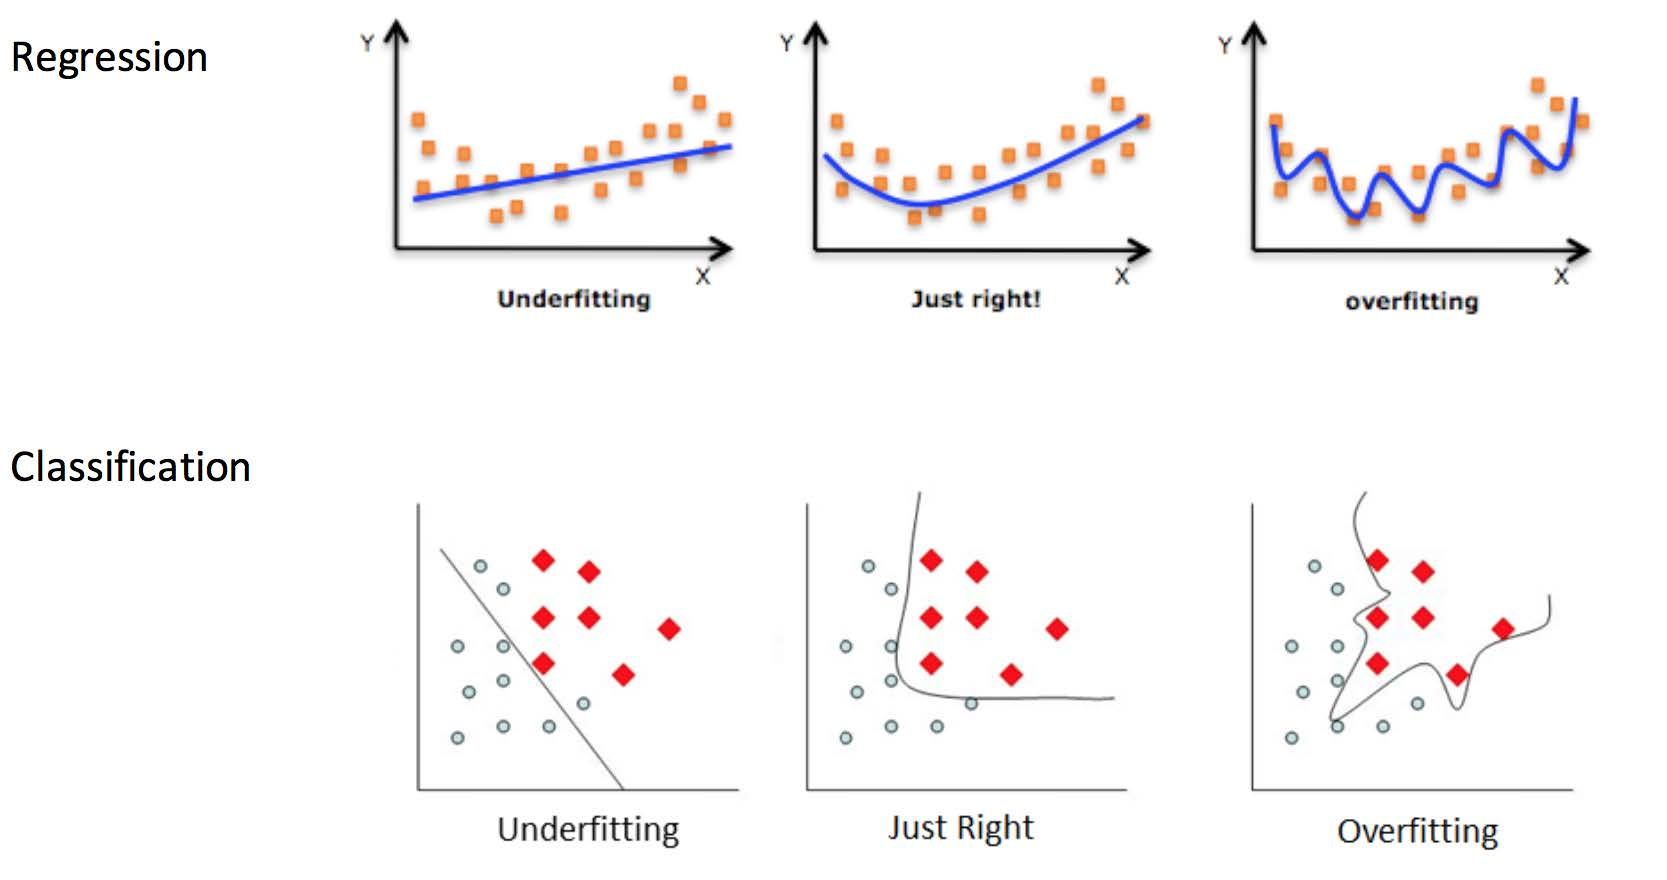
\includegraphics[width=\linewidth]{imgs/intro/overfit}
    \end{center}
    \legend{Fonte: }
    \label{fig:mlflow}
\end{figure}


Enquanto a escolha de um modelo adequado é suficiente para evitar o \textit{underfitting}, diversos fatores contribuem podem contribuir para a ocorrência de \textit{overfitting}. 

\section{Objetivos}

Esse trabalho apresenta um método de seleção de variáveis de entrada para modelos treinados através de aprendizado supervisionado. 

O algoritmo a ser descrito estima o desempenho das variáveis individualmente e em conjunto através do treinamento de modelos lineares e do cálculo de sua performance aplicando a estratégia de validação cruzada.